\chapter{Troubleshooting}
\label{sec:troubleshooting}

\section{Known Issues}

\subsection{CentOS Fuse Usermount Permissions}

On some operating systems, the following error message is shown when starting the AppImage:

\begin{verbatim}
fuse: failed to exec fusermount: Permission denied

Cannot mount AppImage, please check your FUSE setup.
You might still be able to extract the contents of this AppImage 
if you run it with the --appimage-extract option. 
See https://github.com/AppImage/AppImageKit/wiki/FUSE 
for more information
open dir error: No such file or directory
\end{verbatim}


As the message states, the current user has no permissions to correctly mount the AppImage. Please refer to the provded link \url{https://github.com/AppImage/AppImageKit/wiki/FUSE} for information how to resolve this.

\subsection{Missing glibc Library Versions}

On some operating systems, the following error message is shown when starting the AppImage:\\\\

\begin{verbatim}
/lib64/libc.so.6: version `GLIBC_2.14' not found (required by ...)
/usr/lib64/libstdc++.so.6: version `GLIBCXX_3.4.14' not found (required by ...)
/usr/lib64/libstdc++.so.6: version `GLIBCXX_3.4.15' not found (required by ...)
/lib64/libc.so.6: version `GLIBC_2.14' not found 
  (required by /tmp/.mount_COMPASS-XWB8RF/appdir/bin/../lib/libosgDB.so.130)
...
\end{verbatim}

As stated in \url{https://github.com/AppImage/AppImageKit/issues/398}: \\

``...inside the AppImage requires a newer glibc version than is present on your target system (CentOS 6.7 in your example). The recommended way to produce an AppImage that would run on CentOS 6.7 would be to build on CentOS 6.x...''\\\\

Unfortunately this means that for e.g. CentOS 6.* (or older) an AppImage produced using Ubuntu 14.04 will not run, and currently there no plans to build one (unless requested by large number of users).\\

If this is the case for you please comment on \url{https://github.com/hpuhr/COMPASS/issues/35}.


\subsection{White OSGView \& Shader Errors in Console Log}
\label{ref:issue_shaders}

When the OSGView is started on older, unsupported Intel graphics cards the OSGView only show a white window and the following error messages are logged in the console:

\begin{lstlisting}
...
glLinkProgram 0x1af6a320"" FAILED

VERTEX glCompileShader "main(vertex)" FAILED
VERTEX Shader "main(vertex)" infolog:
0:1(10): error: GLSL 3.30 is not supported. Supported versions are: 1.10, 1.20, 1.30, 1.00 ES, 3.00 ES, and 3.10 ES

FRAGMENT glCompileShader "main(fragment)" FAILED
FRAGMENT Shader "main(fragment)" infolog:
0:1(10): error: GLSL 3.30 is not supported. Supported versions are: 1.10, 1.20, 1.30, 1.00 ES, 3.00 ES, and 3.10 ES

Program "" infolog:
error: linking with uncompiled/unspecialized shadererror: linking with uncompiled/unspecialized shadererror: linking with uncompiled/unspecialized shadererror: linking with uncompiled/unspecialized shadererror: linking with uncompiled/unspecialized shadererror: linking with uncompiled/unspecialized shadererror: linking with uncompiled/unspecialized shadererror: linking with uncompiled/unspecialized shadererror: linking with uncompiled/unspecialized shadererror: linking with uncompiled/unspecialized shadererror: linking with uncompiled/unspecialized shadererror: linking with uncompiled/unspecialized shader
glLinkProgram 0x82eefa0"" FAILED
\end{lstlisting}
\ \\

This is due to the the used graphics libraries OpenSceneGraph and osgEarth depending on shaders defined in GLSL 3.30 (shading language version) and the used graphics card driver not supporting this version of shaders. \\

There exists a workaround which might work for you: There exists the issue that in some cases the shaders are supported in the used Mesa graphics driver, but are not detected correctly. One can override the reported OpenGL version for one application using a system variable and start the app in that mode using:

\begin{lstlisting}
MESA_GL_VERSION_OVERRIDE=3.3 ./COMPASS-release.AppImage
\end{lstlisting}

At least on the authors workstation with an Intel graphics card and for some other users this resolved the issue. \\

If this is not the case for you please comment on \url{https://github.com/hpuhr/COMPASS/issues/151}

\subsection{Graphical Issues}

For issues of the following nature:

\begin{itemize} 
\item Application might not even start (OpenGl version error)
\item Slow display performance
\item Graphical display errors (wrong colours, artefacts, etc) 
\end{itemize} 

If such a display issue exists, additional information is required. \\

Please \textbf{verify} that the installed graphics card and driver in use match the supported version stated in \nameref{sec:graphics_installation}. \\

Only if this is the case, please collect the output of \textit{glxinfo} and create an issue report as stated below.

\subsection{ADS-B Target Reports Not Shown}

If imported ADS-B target reports are not displayed in the OSGView, one cause can be that the latitude/longitude position information is only given in it's high precision data item in ASTERIX. So e.g. instead of the 'Latitude' variable, the 'Latitude HP' variable holds the respective information in COMPASS. This could be inspected e.g. using the Histogram or the Scatterplot views. \\

To change the usage of the position information, (once) start the COMPASS application using the '--expert\_mode' command line option, (after opening any database) and step into the Configuration $\rightarrow$ Configure Meta Variables dialog. \\

In said dialog, change both the 'Latiude' and 'Longitude' meta-variables to use the CAT021 'Latitude HP' and 'Longitude HP'.

\begin{figure}[H]
    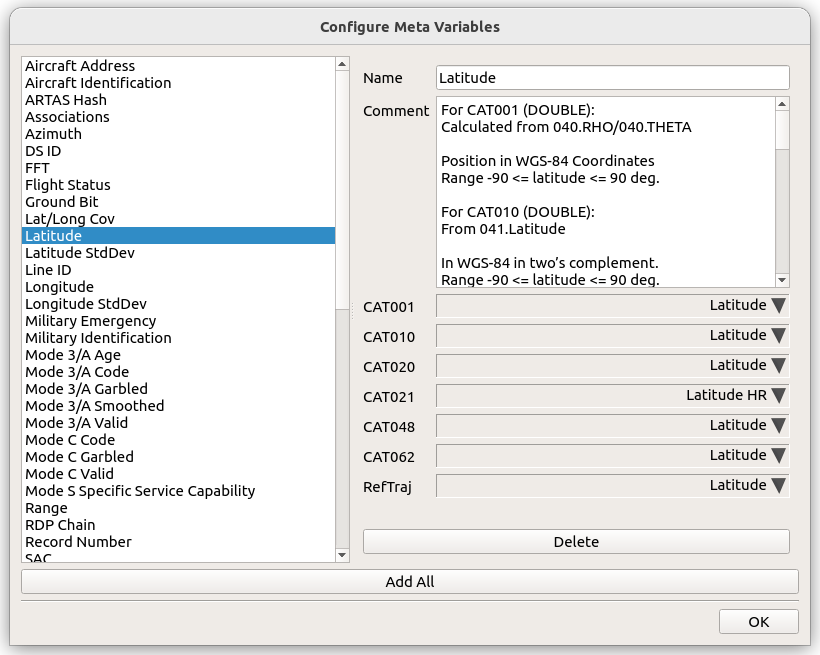
\includegraphics[width=12cm,frame]{figures/meta_latitude_hr.png}
\end{figure}

After these changes, restart the application and (to be safe) re-create the respective database. \\

Please note that, to use the old configuration (e.g. for older ADS-B data) these configuration changes have to be reverted. This issue will be resolved in a future version.



\section{Reporting Issues}

There are several ways of reporting issues. The following steps have to be taken:

\begin{itemize}  
\item Check if the issue was already reported
\item Collect all required information
\item Report the issue
\end{itemize} 

Please also make sure that you are using the latest version of COMPASS, since the issue might already have been corrected in the current version. \\

Also, if you're planning on using COMPASS, it is of benefit if you register on \url{https://github.com}, which can be done for free. It is then possible for you to comment on issues, create new ones or even contribute to the project.

\subsection{Already Reported Issues}

Please refer to \url{https://github.com/hpuhr/COMPASS/issues} for a list of the currently known issues. An issue can be ``Open'' meaning it was not yet fixed, or ``Closed'', meaning it was at least fixed in the source code. If it is closed, it does not mean that the fix is already included in the current AppImage, but that it will be in the next release. \\

Please look through the issues and make sure that yours isn't already listed. If so, you can comment on it to indicate the severity for you. If not, please proceed to the next step.

\subsection{Collect Information}

Basically everything that is needed to reproduce the error should be submitted. Depending on the type of the error, this can differ, but at least the following information should be given:

\begin{itemize}  
\item Console log of the application
\item Exact steps taken until the error occured
\end{itemize} 

\subsubsection{For Application Crashes}

If the application crashed, it would also be of interest to get a stacktrace. This can be achieved by running the application using gdb (\url{https://www.gnu.org/software/gdb/}), which might have to be installed.

Then, the application can be run using ``gdb ./COMPASS-XXX.AppImage''. The output will look similiar to this:

\begin{verbatim}
GNU gdb (Ubuntu 8.0.1-0ubuntu1) 8.0.1
Copyright (C) 2017 Free Software Foundation, Inc.
License GPLv3+: GNU GPL version 3 or later <http://gnu.org/licenses/gpl.html>
This is free software: you are free to change and redistribute it.
There is NO WARRANTY, to the extent permitted by law.  Type "show copying"
and "show warranty" for details.
This GDB was configured as "x86_64-linux-gnu".
Type "show configuration" for configuration details.
For bug reporting instructions, please see:
<http://www.gnu.org/software/gdb/bugs/>.
Find the GDB manual and other documentation resources online at:
<http://www.gnu.org/software/gdb/documentation/>.
For help, type "help".
Type "apropos word" to search for commands related to "word"...
Reading symbols from ./COMPASS-x86_64_RELDBG_0220.AppImage...done.
(gdb) 
\end{verbatim}


In the shown console, enter the command ``run''. This will run the application. Then, perform the same steps as previously to reproduce the application crash.

When the crash occurs, the output should look like this:

\begin{verbatim}
Thread 1 "AppRun" received signal SIGINT, Interrupt.
0x00007fffef950951 in __GI___poll (fds=0x7fffcc007630, nfds=3, timeout=15036) 
at ../sysdeps/unix/sysv/linux/poll.c:29
29	../sysdeps/unix/sysv/linux/poll.c: No such file or directory
\end{verbatim}

Then, enter the command ``backtrace''. This will show output similiar to this:

\begin{verbatim}
#0  0x00007fffef950951 in __GI___poll (fds=0x7fffcc007630, nfds=3, timeout=15036) at 
../sysdeps/unix/sysv/linux/poll.c:29
#1  0x00007fffec5bb169 in ?? () from /lib/x86_64-linux-gnu/libglib-2.0.so.0
#2  0x00007fffec5bb27c in g_main_context_iteration () 
from /lib/x86_64-linux-gnu/libglib-2.0.so.0
#3  0x00007ffff308998c in QEventDispatcherGlib::processEvents
(QFlags<QEventLoop::ProcessEventsFlag>) ()
   from /tmp/.mount_COMPASS-1XB9QP/appdir/bin/../lib/libQt5Core.so.5
#4  0x00007ffff303b96b in QEventLoop::exec(QFlags<QEventLoop::ProcessEventsFlag>)
 () from /tmp/.mount_COMPASS-1XB9QP/appdir/bin/../lib/libQt5Core.so.5
#5  0x00007ffff30420e1 in QCoreApplication::exec() () from 
/tmp/.mount_COMPASS-1XB9QP/appdir/bin/../lib/libQt5Core.so.5
#6  0x00000000006be3c6 in main ()
\end{verbatim}

This is called a stacktrace. Please copy all of this text so that it can be subitted with the issue report.


\subsection{Issue Reporting}

Please either create a new isse on GitHub (\url{https://github.com/hpuhr/COMPASS/issues}) or send a mail to \href{mailto:compass@openats.at}{compass@openats.at}, and include all of the previously collected information. \\

If the supplied information is not enough you will be contacted as soon as time allows, with a request for further detail.


